%-------------------------------------------------------------------------------
\section{Methodology for Analyzing LDAP Security}
\label{sec:methodology}

\begin{figure*}[tb]
\centering 
  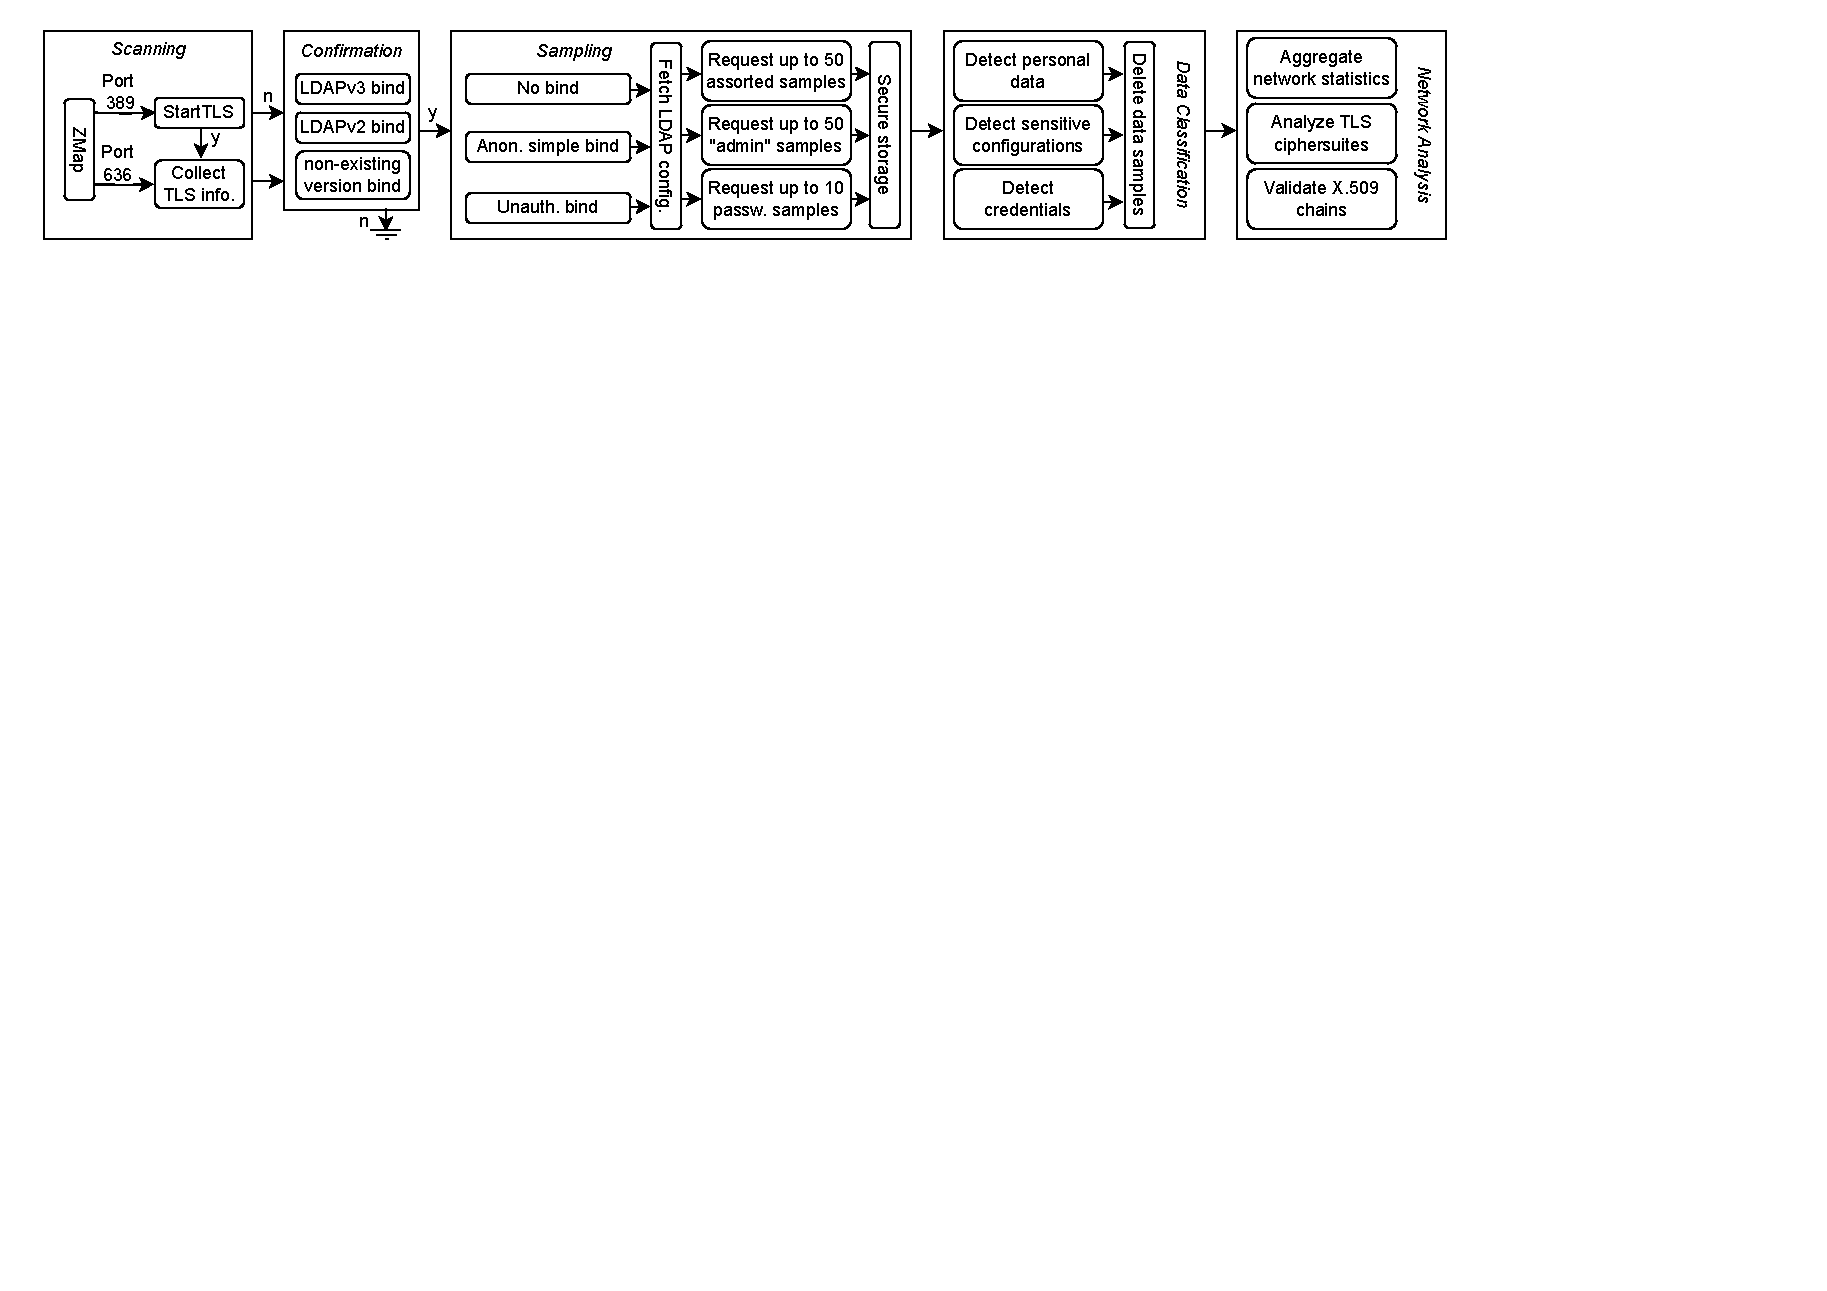
\includegraphics[width=\linewidth]{img/pipeline.pdf}
  
  \caption{\NAME{} analysis pipeline.}
  \label{fig:scanning_pipeline}
\end{figure*} 

\subsection{Threat Model}
We assume that the attackers access publicly available LDAP servers on common ports, \eg by connecting to the IP address of a public LDAP server with a standard LDAP browser. The attackers send standard-conforming packets to retrieve data from LDAP servers and do not attempt to circumvent deployed access controls. Further, we assume they take educated guesses about default configurations---including administrator usernames and attribute names commonly observed. 
% None of these capabilities are restrictive.

When analyzing the security of TLS configurations, we assume that network attackers act as active \gls{MITM} between the LDAP client and server. These attackers aim to exploit weak TLS configurations or downgrade the connection to plaintext to steal the LDAP client's credentials and other sensitive data.

\subsection{\NAME{} Analysis Pipeline Overview}
\NAME{} uses a set of modules for the analysis illustrated in \cref{fig:scanning_pipeline}. This section gives a brief overview of the analysis pipeline. The \emph{scanning module} performs Internet-wide port scans, resulting in a dataset of IPs responding on well-known LDAP ports. It also collects information on TLS configurations on LDAP servers.
Upon detecting an open LDAP port on either of the targeted ports, \NAME's \emph{confirmation module} sends LDAPv2, LDAPv3, or unspecified LDAPv4 messages to provoke an LDAP response.  
The \emph{sampling module} then attempts to connect to identified LDAP servers and performs information requests through standard-conforming connection and anonymous authentication methods. 
If a connection succeeds, the \emph{sampling module} requests configuration settings and metadata. Additionally, it requests a subset of \gls{LDAP} entries from the server for further analysis and stores the data on an internal analysis server.

The two final stages analyze the collected data. The \emph{data classification module} analyzes the configuration details and collected samples for exposed personal data, sensitive data shortcomings, and leakage of credentials. 
The last stage is the \emph{network analysis module}, which analyzes the security of LDAP servers' TLS configurations. 
% found that are not churning. 
The system examines the supported cipher suites and the trust chain.
The  pipeline was executed in January 2024, and we base our evaluation on the data gathered from this run.

%and other statistics, such as issuers and certificate lifespans \rh{At the moment, we don't include these in the paper! So we may need to change the figure and description accordingly.}. 
%Each analysis shows a lack of administration with LDAP servers used to authenticate users, exposing them to the risk of eavesdropping on their communication with servers that contain credentials.

% Figure~\autoref{fig:scanning_pipeline} shows the steps of the LanDscAPe analysis pipeline. The \emph{scanning module} starts by scanning the full IPv4 Internet on ports 389/tcp and 636/tcp (LDAPS) using ZMap~\cite{durumeric2013zmap}. On port 636, it continues with a TLS handshake and collects information about supported TLS versions, supported ciphersuites, and the TLS certificate. On port 389, it issues the StartTLS (Section 3 in \cite{rfc4513}) command to upgrade the plaintext tcp connection to TLS and also collect aforementioned TLS-related information. If an LDAP server has both ports open, there are three possible options to connect to it. First, via a plaintext tcp connection on port 389 with no StartTLS. Second, via an encrypted tcp connection on port 389 with StartTLS, and third, via an encrypted tcp connection on port 636. To reduce stress on scanned networks, we do not attempt to connect to the LDAP server via UDP.

% For each of the mentioned connection types, LanDscAPe's \emph{validation module} attempts three different ways to bind to the LDAP server. First, it attempts to request information from the server with no bind. According to~\cite{rfc4513}, this should bring LanDscAPe to an anonymous authorization identity.
% Second, it attempts to request information with a simple bind using an empty username and empty password field, as specified in section 5.1.1 in~\cite{rfc4513}. Third, it attempts an unauthenticated bind, as specified in section 5.1.2 in~\cite{rfc4513} using an arbitrary username and empty password field. \todo{this is not correct:}If any of these requests results in a response not conforming to the LDAP language specification, it assumes that this server, despite having the appropriate port open, is not an LDAP server. If it received a valid LDAP responses, even valid LDAP error messages, it continues analyzing this server.


% anon We usedeither the  on ports most commonly used for LDAP servers~\cite{censys15, OpenLDAPSoftwareAdministrator26}, 389 and 636. 

% We followed up with a modified version of Goscanner \cite{Goscanner2023} to engage with Start TLS (when applicable) and retrieve the TLS certificates. \cref{fig:scanning_pipeline} depicts the scanning pipeline used to retrieve TLS certificates and identify LDAP servers. The results are stored on the University premises.
%We conducted additional scans to identify different versions of LDAP. We sent an anonymous bind request in LDAPv2 and LDAPv3 to each IP address using the \enquote{python-ldap} Python library \cite{python-ldap}, with a network timeout and operation timeout of 2 seconds. We classify servers that accept the binding or return of an LDAP error message as LDAP servers. For connections that experience timeouts, we cannot definitively determine whether they are LDAP servers.
% -First Scan: May(?) 2023, ZMap scan on port 389 and 636. (How important is the first scan? Do we use this data?)\\
%Second Scan (improved) later more: \\
%- ZMap scan, 09.01.2024 on port 389 and 636\\
%- identifying LDAP servers: \\
%-> Anonymous bind (simple bind with empty username and password), LDAP server has to support the bind operation according to RFC xy, binding two times (first bind with protocol version 2 and second bind with protocol version 3), if bind succeeds -> LDAP server, if bind fails -> interpreting the error message and the cause to determine if server speaks LDAP or not or unknown.
%\todo{FI: I already consolidated this into the ethical considerations}
%Prior to conducting scans and testing servers, we adhered to ethical protocols by formally notifying the administrators at Muenster University of Applied Science, the CERT-Bund of the BSI (Germany's Federal Office for Information Security), and the CERT-DFN of the DFN (German Research Network) about our intended scanning activities. Additionally, as a proactive measure, we employed a blocklist during our scans. This blocklist was based on abuse alerts received from administrators requesting the exclusion of their hosts from the scanning process.
%------------------------------------


\subsection{Scanning Module}

% \rh{I struggled a bit with the level of detail I want to put here to express we had two scanning locations}
% We carry out multiple scans, although we use only the results from \todo{x} scans in this paper. 
% We confirm that the churn rate of \acrshort{LDAP} servers oscillates around 1\% per day; we hence ensure that no scan exceeds 24 hours.

%\item Impl. details
%\item Hardware details \todo{FHMS: Intel(R) Xeon(R) Gold 6240L CPU @ 2.60GHz, 1.5 TB memory, 1 GbE (250 used)---FI: Do we really need to write this?}
%\item Two locations
%\item How long does a scan take? \todo{FHMS: 3 hours per port, well under the normal churn rate} \todo{UT: 23h30m per port (389 and 636, ZMap+Goscanner)}

Our \emph{scanning module} begins by scanning the entire routable IPv4 space on ports TCP/389 and TCP/636 with \zmap ~\cite{durumeric2013zmap}. The former port is used for plain \acrshort{LDAP} and for the in-band upgrade with \starttls, the latter port for \acrshort{LDAP} over TLS. This gives us a list of IPv4 addresses where these ports are open. Previous work~\cite{Izhikevich2022,Sattler2023} shows that many middleboxes will make a port seem open, meaning that the true number of \acrshort{LDAP} servers can only be determined by following through with a higher-layer connection, \ie plain \acrshort{LDAP}, \acrshort{LDAP} and an in-band upgrade to \acrshort{TLS} via \starttls, or a \acrshort{TLS} connection over which an \acrshort{LDAP} connection runs. These are implemented as submodules that execute within 24 hours of the scan. This means that IP churn can lead to us missing an \acrshort{LDAP} host that was still visible in the \zmap scan. We tested the churn and found that it is at most between 1-5\% per day; \eg our \acrshort{TLS} scans always cover at least 95\% of all IP and port combinations (IP:port) for which we also ran successful \acrshort{LDAP} queries. To enable \starttls for \acrshort{LDAP} on port 389, we extend Goscanner~\cite{Goscanner2017} with this form of in-band upgrade to collect connection properties and certificates. On port 636, we connect directly with Goscanner and do a TLS handshake. Goscanner is configured to offer \acrshort{TLS} versions from 1.3 down to 1.0, in that order. A server that supports a more modern version of \acrshort{TLS} should hence select it from our scanner's offer. Similarly, we configured the cipher suites we offer according to the best current practices~\cite{rfc9325}, 
ordered from highly secure to less secure.  However, we do not attempt multiple connections to determine all cipher suites that \acrshort{LDAP} servers support to avoid undue load on them. Note that some servers support both \acrshort{TLS}-protected and plain \acrshort{LDAP} sessions. In our analysis, we treat this case as two distinct ways of accessing a server.

% RH: motivation is not true, and it's already said in limitations
%Note, that the scanning module does not attempt to connect to the \gls{LDAP} server via UDP to reduce stress on scanned networks.
%(react to a TCP SYN packet with a TCP ACK packet) but have not yet established if they are \gls{LDAP} servers.

%We hence connect to each of the (host, port) pairs with  \todo{Gustavo: What is extended, we shall not link to our Github repos}%~\cite{Goscanner2023}
%. On port 636, we connect with \acrshort{TLS} straight-away. On port 389, we connect with plain TCP; the 
%\rh{I think the name of the module is not well chosen; suggest confirmation module or detection module} 
%validation module then sends a \starttls command to upgrade the connection. If supported, we carry out the \acrshort{TLS} handshake and retrieve the certificate chain.
%RH: Are we? \footnoteWe will publish the Goscanner patch with the rest of \NAME.


\subsection{Confirmation Module}
%\rh{Suggest confirmation module as the name}
The \emph{confirmation module} ties directly into the scanning module, but we describe it separately here. It verifies that the candidate IP:port combinations collected in the previous steps actually serve the \gls{LDAP} protocol. To determine this, we send three anonymous simple bind requests with varying versions to each server. First, a normal LDAPv3 bind to check for general LDAP support. Second, an LDAPv2 bind, testing for backward compatibility and outdated servers. Finally, a bind with a non-existing version (v4) to provoke a ``BindResponse where the resultCode is set to protocolError''~\cite{rfc4511}.

If a server does not return a valid LDAP response within five seconds, we abort the attempt. Conversely, if the server replies with an RFC 4513-conforming LDAP message~\cite{rfc4513}, we classify the service as an LDAP server. If no protocol error is encountered, we assume that the server supports the respective LDAP version.

After this step, for each IP:port tuple, we know if they are standard \gls{LDAP} servers, which LDAP versions and connection security they support, and which TLS certificates are used.

\subsection{Sampling Module}
\label{subsec:samplingModule}

The \emph{sampling module} gathers information in a three-step process: connecting to an LDAP server, fetching configuration data and metadata, and collecting sample entries.

\paragraph{Connecting to Servers.} For each server with each supported connection type (port 389 with and without \starttls, and port 636 with implicit TLS), we initially request information without bind, leading to an anonymous authorization identity, according to Section 4 of~\cite{rfc4513}. Subsequently, it executes a simple bind request with both username and password fields left empty, aligning with the specifications in Section 5.1.1 of~\cite{rfc4513}. The third approach involves an unauthenticated bind, as outlined in Section 5.1.2 of~\cite{rfc4513}, using an arbitrary username (we chose \texttt{cn=*}) and an empty password field. We do this for all available connection types per IP address as it may serve different \gls{LDAP} services or configurations on each. 

\paragraph{Fetching Configurations.} Next, we collect configuration information and metadata from the server. We first request the root \gls{DSE} that contains information on supported \gls{LDAP} controls, extensions, features, and versions. Additionally, it contains the server's naming contexts. Based on this, we request the server's schema, size limit, and password policies. 


\paragraph{Collecting Samples.} To assess the data the server publicly exposes, we collect a specific number of entries from the server. To retrieve entries from an \gls{LDAP} server, the client sends an \gls{LDAP} \texttt{SearchRequest} and gets the result via the server's \texttt{SearchResultEntry} response.

For our analysis, we request random, admin, and password samples. We request random samples by sending a query filtering for \texttt{objectClass=*} and admin samples by filtering for \texttt{cn=*admin*}. To prevent the server from sending excessive data, we limit each search to a maximum of 50 entries. For password samples, we request the following fields: \texttt{userpassword}, \texttt{password}, \texttt{sambantpassword}, \texttt{sambalmpassword}, \texttt{krbprincipalkey}, \texttt{clearpassword}, \texttt{goimappassword}, \texttt{lmpassword}, and \texttt{ntpassword}.
Here, we limit each request to a maximum of ten results. For ethical reasons, we do not make further requests and accept a smaller sample size if the server responds with less.

\paragraph{Secure Data Storage.} Even though we only sample public LDAP servers, collected data samples may contain sensitive information as critical as user credentials. To protect these samples, this module moves them from the scanning server to an internal server that is only accessible via VPN by the researchers involved in this analysis.

\subsection{Data Classification Module}
\label{sec:methodology_data_analysis_module}

The \emph{data classification module} tries to identify the types of data samples collected in earlier stages. Particularly, it aims to detect personal data, internal information, and credentials within our samples. In its final step, all samples are deleted, and only metadata indicating the type of data found per server is kept to prevent possible harm from unauthorized access.

\paragraph{Detect Personal Data.}

We analyze our samples for typical personal data attributes such as names, email addresses, or certificates. We follow Art. 4 of the \acrshort{GDPR} here that defines personal data as any information relating to an identified or identifiable natural person~\cite[Art. 4]{GDPR2016a}. To identify personal data, we first aggregate semantically identical attributes of our samples (max. 50 samples per server, less if the server sends less), \eg attributes such as \texttt{surname}, \texttt{sn} and \texttt{lastname} (see Table \ref{tab:personal_data_attribute_groups} for more details). We then group by this aggregation and count the servers containing personal data.  

\paragraph{Detect Sensitive Configurations.}

We try to identify potentially insecure servers and confidential information on servers. Therefore, we first categorize LDAP servers into usage scenarios and common products. This categorization uses three indicators: OIDs, the root \gls{DSE} \texttt{vendorName} and \texttt{vendorVersion} fields, and random sample attributes with hints such as the \texttt{msExch} prefix referencing an AD. Since some servers communicate their exact version, we look up the corresponding version number on~\cite{security_vulnerability_database}. However, this is only a weak indicator that the vulnerability is exploitable and harms the overall security. 

Furthermore, we look at \gls{SASL} mechanisms supported by servers. While some mechanisms are notably secure, \eg using salts or providing memory or CPU hardness, others are not. If LDAP servers act as authentication servers, a strong \gls{SASL} configuration is important.

Moreover, we consider servers exposing internal information related to LinuxUserManagement, Microsoft Active Directory, DICOM, and \texttt{passwordPolicies} having a sensitive configuration. If this information is publicly accessible (\eg \texttt{gidNumber}, \texttt{uidNumber}), it might be utilized by attackers.

\paragraph{Credentials Detection.}

To detect user credentials on LDAP servers, we examine our fetched password samples (max. 10 samples per password field, less if the server sends less, see section \ref{subsec:samplingModule}) and evaluate their values. We automate this process using tags according to~\cite{OpenLDAPSoftwareAdministrator} and pattern recognition (\eg BCRYPT). If we detect encodings such as base64, we try automatically to decode and restart the evaluation process. If the password type of a value was not recognizable (\eg password was masked with asterisks), we excluded the server from further analysis. To assess the extent of leaked passwords, we proceed by reconnecting to the server and counting the number of entries that contain a non-empty password field without transferring any further sensitive information by restricting the attributes returned by the server to the \texttt{DN}. We do this by setting the requested attribute list to empty as shown in \cref{lst:generic_query}.
%We set the attributes parameter to an empty array, ensuring that only the \texttt{dn} attribute is returned in the search results.
We have taken these steps to transfer minimal sensitive information minimizing the risk for users.

\begin{lstfloat}[bt]
\setlength{\belowcaptionskip}{-1em}
\begin{lstlisting}[basicstyle=\ttfamily\footnotesize, frame=single]
def generic_query(prefix):
    results = []
    for letter in alphabet:
        filter=f"(&(cn={prefix + letter}*)(userPassword=*))"
        try:
            result=ldap_connection.search(filter,attributes=[])
        except SIZELIMIT_EXCEEDED:
            result=generic_query(prefix + letter)
        results.extend(result)
    return results
\end{lstlisting}
\caption{Prefix search to count LDAP entries.}
\label{lst:generic_query}
\end{lstfloat}

\paragraph{Data Deletion.}
The module only collects and retains information about the type of data available on any public LDAP server. To minimize risk for organizations and users, we delete all collected samples when this module finishes.

\begin{table*}[tb]
\newcommand{\goodtls}{\multicolumn{1}{c}{\normalsize\usym{1F512}}}
\newcommand{\badtls}{\multicolumn{1}{c}{\normalsize\usym{1F513}}}
\newcommand{\notls}{\multicolumn{1}{c}{\normalsize\usym{1F6AB}}}
\newcommand{\plainpwd}{\multicolumn{1}{c}{Plain}}
\newcommand{\hashedpwd}{\multicolumn{1}{c}{Hashed}}
%\setlength\tabcolsep{3.5pt}
\footnotesize
    \centering
    \begin{tabular}{@{} l r r r r rrr @{}}
         \toprule
                 \multirow{2}{*}{\thead{Region}}&\multirow{2}{*}{\thead{Total IPs}}&{\thead{Per 1M}}&\thead{Leaking} & \multirow{2}{*}{\thead{Personal Data}} & \multicolumn{3}{c}{\thead{Sensitive LDAP Configuration}}\\
                 \cline{6-8}\noalign{\vspace{0.5ex}}
         & &  \thead{inhabitants} &\thead{Credentials}&& \multicolumn{1}{@{}l}{\thead{SASL Support}} & \thead{CVE Exists} & \thead{Internal Info.}\\
         \midrule
         \midrule
World &82,129 (100\%) & 46 & 1,817 (2.21\%) & 12,179 (14.83\%) & 26,464 (32.22\%) & 616 (0.75\%) & 9,731 (11.85\%)\\
         \arrayrulecolor{gray!90}
         \midrule
         \arrayrulecolor{black}
% United States&18,466 (22.48 \%) & 56 & 463 (2.51 \%) & 2,968 (16.07 \%) & 4,995 (27.05 \%) & 1,744 (9.44 \%) & 204 (1.10 \%)\\
% Germany&8,123 (9.89 \%) & 97 & 77 (0.95 \%) & 872 (10.73 \%) & 2,138 (26.32 \%) & 671 (8.26 \%) & 48 (0.59 \%)\\
% France&5,122 (6.24 \%) & 78 & 95 (1.85 \%) & 888 (17.34 \%) & 1,833 (35.79 \%) & 632 (12.34 \%) & 25 (0.49 \%)\\
% Poland&5,040 (6.14 \%) & 133 & 27 (0.54 \%) & 153 (3.04 \%) & 708 (14.05 \%) & 144 (2.86 \%) & 8 (0.16 \%)\\
% Russia&4,042 (4.92 \%) & 28 & 36 (0.89 \%) & 406 (10.04 \%) & 1,112 (27.51 \%) & 389 (9.62 \%) & 39 (0.96 \%)\\
% China&4,004 (4.88 \%) & 3 & 369 (9.22 \%) & 812 (20.28 \%) & 1,037 (25.90 \%) & 729 (18.21 \%) & 33 (0.82 \%)\\
% United Kingdom&2,724 (3.32 \%) & 40 & 12 (0.44 \%) & 230 (8.44 \%) & 452 (16.59 \%) & 139 (5.10 \%) & 12 (0.44 \%)\\
% Taiwan&2,717 (3.31 \%) & 113 & 24 (0.88 \%) & 383 (14.10 \%) & 1,027 (37.80 \%) & 203 (7.47 \%) & 3 (0.11 \%)\\
% Brazil&2,656 (3.23 \%) & 12 & 57 (2.15 \%) & 232 (8.73 \%) & 583 (21.95 \%) & 269 (10.13 \%) & 4 (0.15 \%)\\
% India&2,583 (3.15 \%) & 2 & 89 (3.45 \%) & 356 (13.78 \%) & 875 (33.88 \%) & 388 (15.02 \%) & 5 (0.19 \%)\\
% Italy&2,545 (3.10 \%) & 42 & 46 (1.81 \%) & 411 (16.15 \%) & 672 (26.40 \%) & 281 (11.04 \%) & 19 (0.75 \%)\\
% Netherlands&2,260 (2.75 \%) & 132 & 18 (0.80 \%) & 187 (8.27 \%) & 498 (22.04 \%) & 162 (7.17 \%) & 16 (0.71 \%)\\
% Canada&2,027 (2.47 \%) & 54 & 14 (0.69 \%) & 384 (18.94 \%) & 769 (37.94 \%) & 291 (14.36 \%) & 13 (0.64 \%)\\
% Switzerland&1,548 (1.88 \%) & 179 & 9 (0.58 \%) & 116 (7.49 \%) & 202 (13.05 \%) & 74 (4.78 \%) & 11 (0.71 \%)\\
% Indonesia&1,479 (1.80 \%) & 5 & 17 (1.15 \%) & 127 (8.59 \%) & 1,023 (69.17 \%) & 482 (32.59 \%) & 4 (0.27 \%)\\
% Vietnam&1,462 (1.78 \%) & 15 & 6 (0.41 \%) & 81 (5.54 \%) & 545 (37.28 \%) & 308 (21.07 \%) & 1 (0.07 \%)\\
% Japan&1,338 (1.63 \%) & 11 & 93 (6.95 \%) & 289 (21.60 \%) & 318 (23.77 \%) & 184 (13.75 \%) & 27 (2.02 \%)\\
% South Africa&1,200 (1.46 \%) & 20 & 1 (0.08 \%) & 54 (4.50 \%) & 116 (9.67 \%) & 28 (2.33 \%) & 5 (0.42 \%)\\
% South Korea&1,179 (1.44 \%) & 23 & 43 (3.65 \%) & 201 (17.05 \%) & 319 (27.06 \%) & 195 (16.54 \%) & 5 (0.42 \%)\\
% Australia&1,032 (1.26 \%) & 40 & 15 (1.45 \%) & 104 (10.08 \%) & 203 (19.67 \%) & 85 (8.24 \%) & 6 (0.58 \%)\\
% Thailand&1,019 (1.24 \%) & 15 & 16 (1.57 \%) & 73 (7.16 \%) & 326 (31.99 \%) & 183 (17.96 \%) & 6 (0.59 \%)\\
% Hong Kong&918 (1.12 \%) & 122 & 28 (3.05 \%) & 109 (11.87 \%) & 281 (30.61 \%) & 161 (17.54 \%) & 9 (0.98 \%)\\
% Czechia&909 (1.11 \%) & 85 & 21 (2.31 \%) & 149 (16.39 \%) & 308 (33.88 \%) & 114 (12.54 \%) & 21 (2.31 \%)\\
% Singapore&837 (1.02 \%) & 143 & 22 (2.63 \%) & 134 (16.01 \%) & 384 (45.88 \%) & 135 (16.13 \%) & 7 (0.84 \%)\\
% Spain&821 (1.00 \%) & 18 & 9 (1.10 \%) & 127 (15.47 \%) & 302 (36.78 \%) & 90 (10.96 \%) & 3 (0.37 \%)\\
United States&18,466 (22.48 \%) & 56 & 463 (2.51 \%) & 2,968 (16.07 \%) & 4,995 (27.05 \%) & 204 (1.10 \%) & 1,744 (9.44 \%)\\
Germany&8,123 (9.89 \%) & 97 & 77 (0.95 \%) & 872 (10.73 \%) & 2,138 (26.32 \%) & 48 (0.59 \%) & 671 (8.26 \%)\\
France&5,122 (6.24 \%) & 78 & 95 (1.85 \%) & 888 (17.34 \%) & 1,833 (35.79 \%) & 25 (0.49 \%) & 632 (12.34 \%)\\
Poland&5,040 (6.14 \%) & 133 & 27 (0.54 \%) & 153 (3.04 \%) & 708 (14.05 \%) & 8 (0.16 \%) & 144 (2.86 \%)\\
Russian Federation&4,042 (4.92 \%) & 28 & 36 (0.89 \%) & 406 (10.04 \%) & 1,112 (27.51 \%) & 39 (0.96 \%) & 389 (9.62 \%)\\
China&4,004 (4.88 \%) & 3 & 369 (9.22 \%) & 812 (20.28 \%) & 1,037 (25.90 \%) & 33 (0.82 \%) & 729 (18.21 \%)\\
United Kingdom&2,724 (3.32 \%) & 40 & 12 (0.44 \%) & 230 (8.44 \%) & 452 (16.59 \%) & 12 (0.44 \%) & 139 (5.10 \%)\\
Taiwan &2,717 (3.31 \%) & 113 & 24 (0.88 \%) & 383 (14.10 \%) & 1,027 (37.80 \%) & 3 (0.11 \%) & 203 (7.47 \%)\\
Brazil&2,656 (3.23 \%) & 12 & 57 (2.15 \%) & 232 (8.73 \%) & 583 (21.95 \%) & 4 (0.15 \%) & 269 (10.13 \%)\\
India&2,583 (3.15 \%) & 2 & 89 (3.45 \%) & 356 (13.78 \%) & 875 (33.88 \%) & 5 (0.19 \%) & 388 (15.02 \%)\\
Italy&2,545 (3.10 \%) & 42 & 46 (1.81 \%) & 411 (16.15 \%) & 672 (26.40 \%) & 19 (0.75 \%) & 281 (11.04 \%)\\
Netherlands&2,260 (2.75 \%) & 132 & 18 (0.80 \%) & 187 (8.27 \%) & 498 (22.04 \%) & 16 (0.71 \%) & 162 (7.17 \%)\\
Canada&2,027 (2.47 \%) & 54 & 14 (0.69 \%) & 384 (18.94 \%) & 769 (37.94 \%) & 13 (0.64 \%) & 291 (14.36 \%)\\
Switzerland&1,548 (1.88 \%) & 179 & 9 (0.58 \%) & 116 (7.49 \%) & 202 (13.05 \%) & 11 (0.71 \%) & 74 (4.78 \%)\\
Indonesia&1,479 (1.80 \%) & 5 & 17 (1.15 \%) & 127 (8.59 \%) & 1,023 (69.17 \%) & 4 (0.27 \%) & 482 (32.59 \%)\\
Viet Nam&1,462 (1.78 \%) & 15 & 6 (0.41 \%) & 81 (5.54 \%) & 545 (37.28 \%) & 1 (0.07 \%) & 308 (21.07 \%)\\
Japan&1,338 (1.63 \%) & 11 & 93 (6.95 \%) & 289 (21.60 \%) & 318 (23.77 \%) & 27 (2.02 \%) & 184 (13.75 \%)\\
South Africa&1,200 (1.46 \%) & 20 & 1 (0.08 \%) & 54 (4.50 \%) & 116 (9.67 \%) & 5 (0.42 \%) & 28 (2.33 \%)\\
South Korea &1,179 (1.44 \%) & 23 & 43 (3.65 \%) & 201 (17.05 \%) & 319 (27.06 \%) & 5 (0.42 \%) & 195 (16.54 \%)\\
Australia&1,032 (1.26 \%) & 40 & 15 (1.45 \%) & 104 (10.08 \%) & 203 (19.67 \%) & 6 (0.58 \%) & 85 (8.24 \%)\\
Thailand&1,019 (1.24 \%) & 15 & 16 (1.57 \%) & 73 (7.16 \%) & 326 (31.99 \%) & 6 (0.59 \%) & 183 (17.96 \%)\\
Hong Kong&918 (1.12 \%) & 122 & 28 (3.05 \%) & 109 (11.87 \%) & 281 (30.61 \%) & 9 (0.98 \%) & 161 (17.54 \%)\\
Czech Republic &909 (1.11 \%) & 85 & 21 (2.31 \%) & 149 (16.39 \%) & 308 (33.88 \%) & 21 (2.31 \%) & 114 (12.54 \%)\\
Singapore&837 (1.02 \%) & 143 & 22 (2.63 \%) & 134 (16.01 \%) & 384 (45.88 \%) & 7 (0.84 \%) & 135 (16.13 \%)\\
Spain&821 (1.00 \%) & 18 & 9 (1.10 \%) & 127 (15.47 \%) & 302 (36.78 \%) & 3 (0.37 \%) & 90 (10.96 \%)\\
         \bottomrule
    \end{tabular}
    %\begin{tabular}{ l l l l }
    %\toprule
    %\goodtls & Proper TLS\\
    %\badtls & Improper TLS\\
    %\notls & Only in plaintext\\
    %\bottomrule
    %\end{tabular}
    \caption{Overview of the results of the Data Analysis Modules grouped by region, sorted by total, top 25 regions. Percentages are based on total servers in the region. 
    %\todo{Are these numbers really consistent with the text?}
    }
    \label{tab:results_overview}
\end{table*}
\subsection{Network Analysis Module}
\label{subsec:methodology_tls_certs}

This module analyzes \acrshort{TLS} cipher suites and the X.509 certificate chains in the \acrshort{TLS} handshakes; it also provides access to aggregate statistics enriched with third-party data sources, such as IP2Location\footnote{\url{https://www.ip2location.com}} to determine the geographical location and hosting situation of an \acrshort{LDAP} instance. For the purpose of this paper, we present only analyses for \acrshort{LDAP} servers with security-relevant properties, \eg those that support authentication via the \acrlong{SASL} framework or host personal data or user credentials. Such servers should use secure \acrshort{TLS} configurations: even if the data can be queried anonymously, it may cross other networks and should hence be protected against privacy-invasive monitoring (\eg queries to a public address book will reveal the communication behavior of individuals). We define ``secure'' by referring to the best-practice recommendations for \acrshort{TLS} in RFC 9325 \cite{rfc9325} for connections and X.509 certificate chains.
%Such secure \acrshort{TLS} we refer to as without issues. 
The server chooses the cipher suite from a list the client offers; we can obtain the chosen cipher suite from the handshake.

The certificates need to be validated against root stores that contain the public keys of recognized certificate issuers, \ie Certificate Authorities (CAs). For the Web PKI, such certificate stores are well-known and can be downloaded for browsers and operating systems. For \acrshort{LDAP}, no defined set of CAs exists. Hence, we check against a ``meta root-store'' and validate the \acrshort{LDAP} certificates against the combined root stores from Apple, Microsoft, Google, CCADB (Mozilla), and Oracle (Java). Together, these are known to cover the majority of \acrshort{TLS} user agents for web users~\cite{maTracingYourRoots2021}. We define a valid chain as one that is valid for at least one root store.

Various problems with certificate chains have been found, initially for the Web~\cite{holz2011,Durumeric2013} and later for other communication protocols, especially email~\cite{holz2016}. The use case of LDAP is different from these protocols: both the Web and email servers are, almost by definition, meant for public access. LDAP is commonly used in ways that are internal to an organization. Hence, there are two choices to configure X.509: either by using a certificate from a globally acting CA or by running a custom, ``in-house'' CA. The former method has the advantage that it is thoroughly documented and certificates are available at no cost from CAs like Let's Encrypt. The latter method also avoids costs, but it comes with more administrative overhead as the local CA must be operated securely by the organization (tooling is available in some environments, \eg Microsoft Windows servers) and its root certificate deployed to client software. In theory, self-signed certificates could also be used to replace an in-house CA; in this case, one would need to ship the self-signed certificate with the client (and possibly alter the software to accept such certificates).

We call certificate chains \textit{globally invalid} if the root CA is
not in the root store. This means that our estimate for the number of valid certificates is a \textit{lower bound} (and an upper bound for the number of invalid chains). Custom CAs can be expected to issue relatively few certificates (as there are few servers per organization).
Independently of these considerations, we always call a chain invalid if there is a cryptographic problem, \eg use of the deprecated SHA1 algorithm for certificate signatures. Our validator uses the standard Go library, which rejects
such certificates as invalid.

Note that we cannot validate the names in the certificates, as the domain names that resolve to an IP are unknown.\footnote{While some large DNS datasets exist (\eg OpenINTEL), these do not cover subdomains, which are likely names for \acrshort{LDAP} servers.}
%Furthermore, we do not test certificate revocation. %Hence, our validation of certificates may paint a too-optimistic picture.

%which leaked passwords and PII, with all LDAP servers on static IP addresses. 
%Our reasoning here is that LDAP servers with PII, user credentials, with SASP support should only be accessed using secure channels. 
%\todo{Gustavo`: What if one trust chain is valid and one is not? - See if I answered it below} 
%We used the Go "x509/crypto", which follows the X.509 standards in the RFC-5280~\cite{rfc5280} and is restricted by CA/Browser Forum Baseline Requirements.
 
 %We verify the certificate chains for all LDAP servers against each different root store, and we define it as valid if the chain is valid in at least one root store. Our tool %verifies certificates apart from the LDAP scanning, \ie, offline. We did not use the certificate subject name since we have not followed up on domain names.
%In this paper, we do not consider \glspl{CRL} and \glspl{OCSP}; hence, we provide a lower bound of invalid certificates.




    